%% Factsheet template for NTIRE 2022 challenge
%% 
%%

\documentclass{article}
\usepackage{bbm}
\usepackage{graphicx}
\usepackage{hyperref}
\title{PoNet+: A Physical Optimization-based Network with Spectral Grouping for Spectral Recovery}
\author{Jiang He, Yi Xiao, Jiajun Xiao, Qiangqiang Yuan, Jie Li, Liangpei}
\begin{document}

\maketitle

\section{Team details}

\begin{itemize}
\item Team name: SGG\_RS\_Whu                                  
\item Team leader name: Jiang He                           
\item Team leader address: School of Geodesy and Geomatics, Wuhan University, Hubei, 430079, China;  \\Phone number: +86 16607114843; Email: jiang\_he@whu.edu.cn; 
\item Yi Xiao(xy574475@gmail.com), Jiajun Xiao(wuhansunyat@gmail.com),\\Qiangqiang Yuan(yqiang86@gmail.com), Jie Li(jli89@sgg.whu.edu.cn), \\Liangpei Zhang(zlp62@whu.edu.cn)
\item School of Geodesy and Geomatics, Wuhan University, China
\item User names: hj\_whu 
\item Best scoring entries of the team during development/validation phase: 0.260699857
\item Link to the codes: \href{https://github.com/JiangHe96/PoNet_plus}{https://github.com/JiangHe96/PoNet\_plus}
\item Link to the restoration results: \href{https://zenodo.org/record/6394053}{https://zenodo.org/record/6394053}
\end{itemize}

\section{Contribution details}

\begin{itemize}
\item PoNet+: A Physical Optimization-based Network with Spectral Grouping for Spectral Recovery                                 
\item A physical optimization-based spectral recovery methods is unrolled into an end-to-end CNN as our previous work PoNet \cite{ponet}. Besides, we employed the spectral grouping similar to HSRnet \cite{hsrnet}. Detialed contributions are shown in below:
\subsection{Physical Optimization Unrolling}
\begin{figure}[!h]
	\centering
	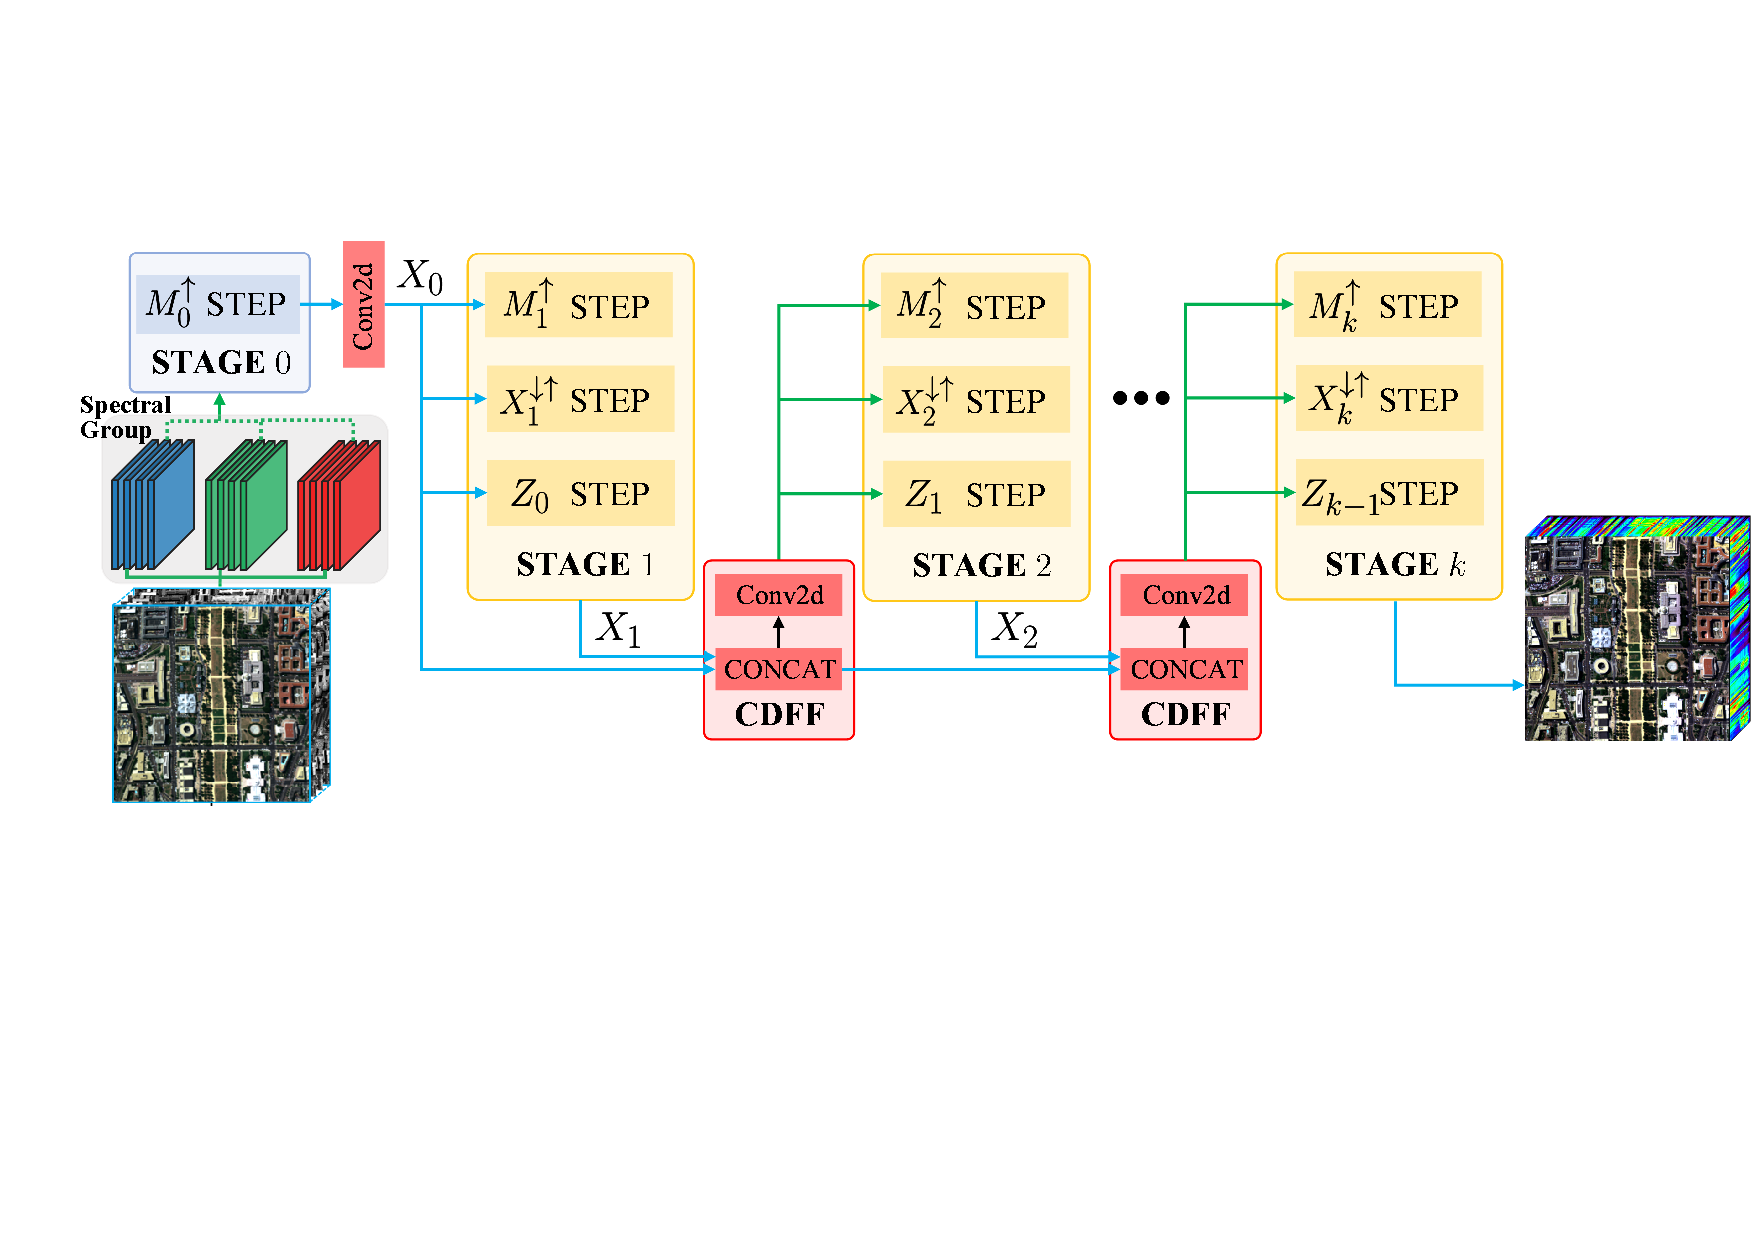
\includegraphics[width=\linewidth]{framework.pdf}
	\caption{The framework of the proposed PoNet+}
	\label{fig1}
\end{figure} 
\par{Let $X\in\mathbbm{R}^{W\times H\times C}$ represent the observed HSI, where C is the number of the spectral channels, and W and H are the width and height, respectively. $Y\in\mathbbm{R}^{W\times H\times c}$ represents the observed multispectral image, where $c<C$ is the number of multispectral bands, specifically for RGB image, with $c=3$. Varying in SRF, the sensors obtain different MS or HS data with different bands.  A  transformation  matrix $\Phi\in\mathbbm{R}^{c\times C}$can be used to describe the spectral degradation between MS and HS imaging as follows.   
}
\begin{equation}
	Y=\Phi X
\end{equation}
\par{The high-dimension HSIs can be approximately predicted by adopting some priors to a minimization problem to constrain the solution space as follows:
}
\begin{equation}
	\hat{{X}}={\arg\min}_X\left\| Y-\Phi{X}\right\|  _{2}^{2}+\lambda\mathcal{R}({X})
\end{equation}
\par{where $\lambda$ is a trade-off parameter, and $\mathcal{R}(\cdot)$ is a regularization function. Employ the half-quadratic splitting method with a penalty parameter as $\mu$ and solve it by the gradient descent algorithm:
}
\begin{equation} 
\hat{{X}}_{k+1} = \left(1-\epsilon\mu\right){X}_k-\epsilon {X}_k{\Phi}{\Phi}^T+\epsilon {M_H}{\Phi}^T+\epsilon\mu{Z}_k
\end{equation}
\begin{equation}
\hat{{Z}}_{k}={Prox}(X_{k})={\arg\min}_Z\left\|{Z}-{X}_{k}\right\| _{2}^{2}+\frac{\lambda}{\mu}\mathcal{R}({Z})
\label{eq8}
\end{equation}
\par\noindent{where $\epsilon$ is the optimization stride. As for the $Z$-subproblem, proximal operators that impose prior knowledge can deal with it.}
\par{Unrolling the physical optimization method into CNN, the proposed PoNet+ is shown in Fig. \ref{fig1}.
}
           

\subsection{Cross-Dimensional Channel Attention}
\par{In traditional physical optimization-based algorithms, hyperparameters need to be defined manually and adjust to the optimal through a large number of experiments. Furthermore, in spectral super-resolution, differential treatment should be performed for the hyperparameters of different channels due to the different radiation characteristics.}
\par{Pooling is a common operation used in traditional channel attention, which is popular for fast computation and no parameter requirement at the cost of high information loss. Furthermore, traditional channel attention weights the different channels of features separately ignoring the interaction between channels. There have been many works stated that building relationships between every two channels is much of importance. However, when the number of channels is large and attention mechanisms are frequently employed, the problem of computational burden should also be focused on.}
\par{Inspired by the above-mentioned points, we proposed a strategy named \textit{Cross-Dimensional Channel Attention} (CDCA) employing 1D and 2D convolutional layers to manage the hyperparameter learning in this paper. 2D convolutional layers are used to extract pixel-by-pixel attention maps. On the other hand, 1D convolutional layers are employed to integrate attention maps for fast computational speed. Details of the proposed module are shown in Fig.~\ref{fig2}.}
\begin{figure}[!h]
	\centering
	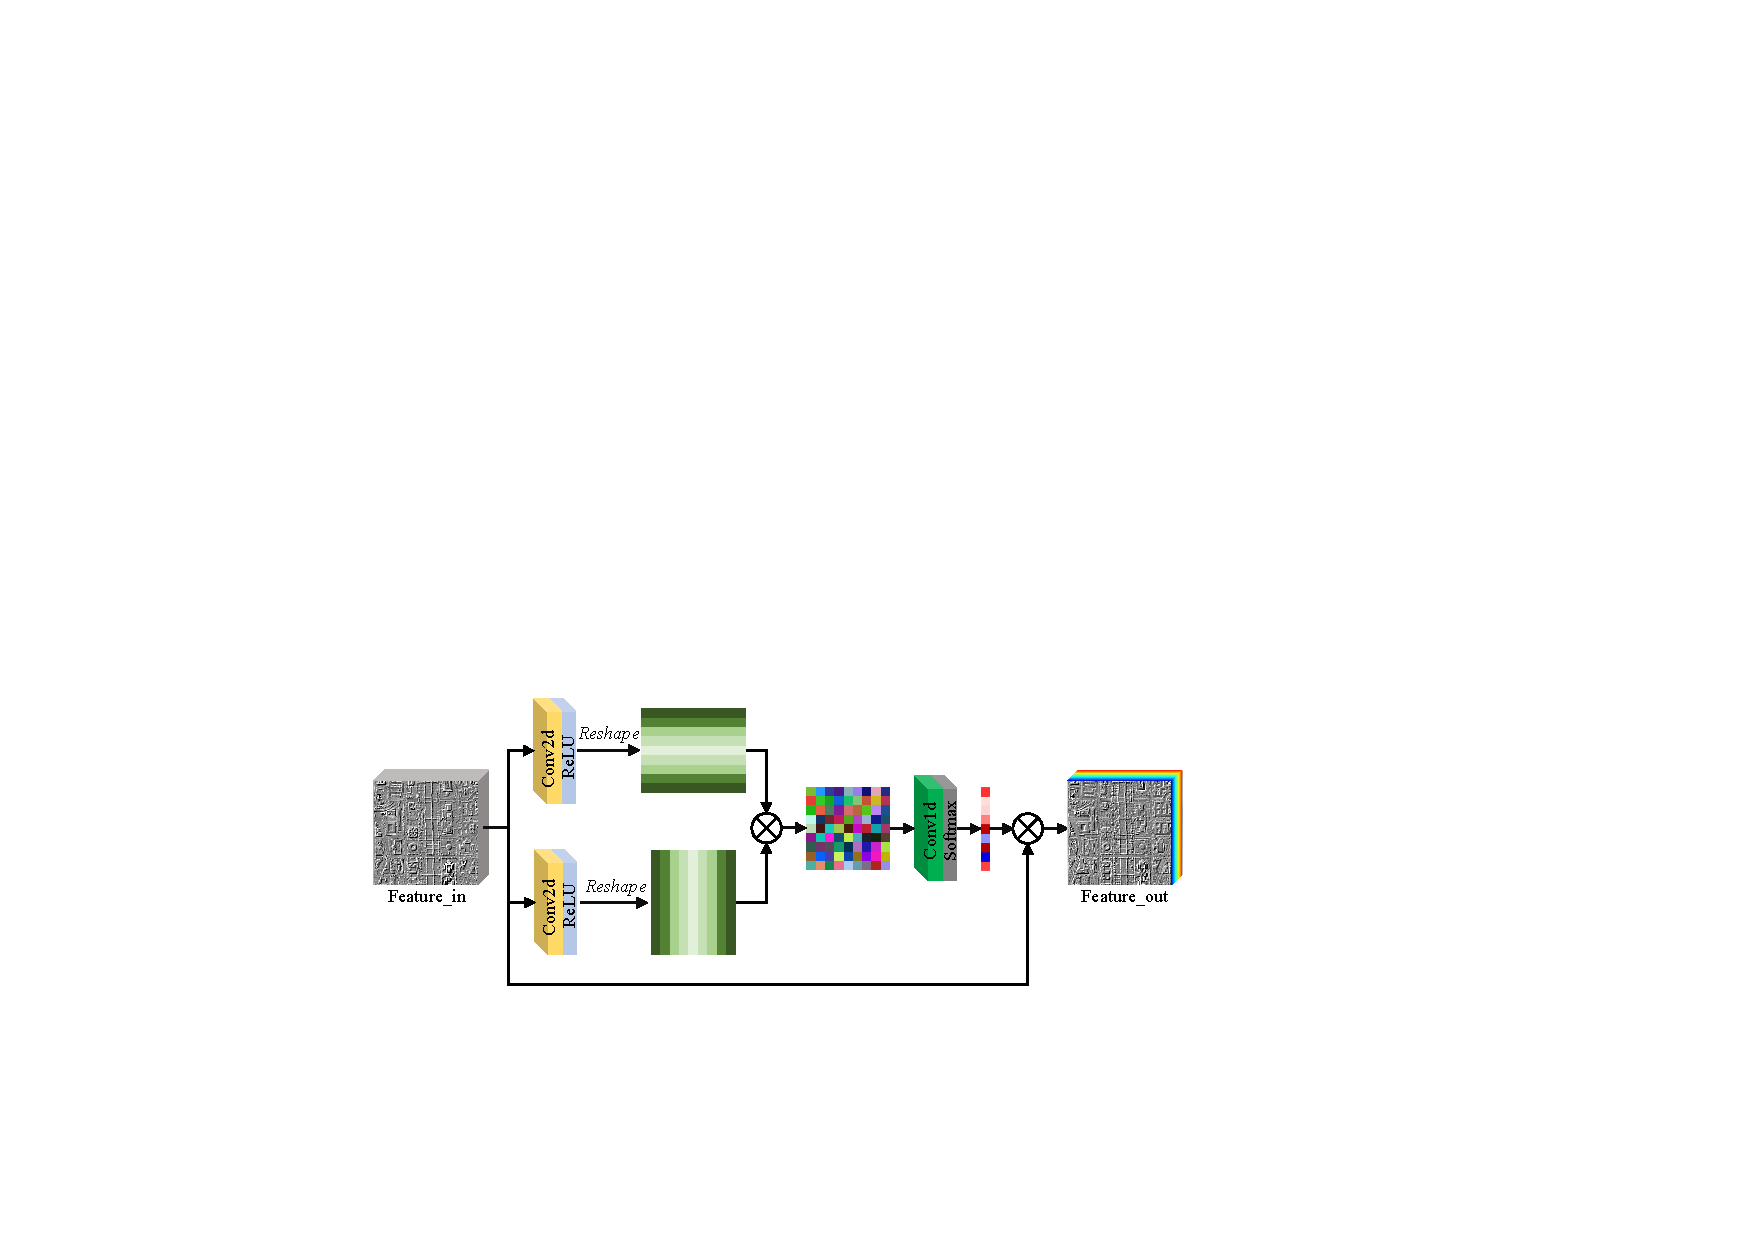
\includegraphics[width=35em]{CDCA.pdf}
	\caption{Cross-dimensional channel attention}
	\label{fig2}
\end{figure}
\par{We adopt two 2D convolutional layers with the kernel size of $1\times1$ to extract different spectral features $R, S\in\mathbbm{R}^{W\times H\times C}$. Attention map $A\in\mathbbm{R}^{C\times C}$ between any two channels can be calculated as follows:}
\begin{equation}
a_{ij}=R_iS_j^T
\end{equation}
\par\noindent{where $a_{ij}$ measures the attention between the $i^{th}$ and $j^{th}$ bands. $R_i$ and $S_j$ is the reshaped channel. To boost the computational speed, we employ a 1D convolutional layer with the kernel size of $k$ to integrate channel-to-channel attention map $A$. Then, the final cross-dimensional channel attention-based hyperparameter $P\in\mathbbm{R}^{1\times C}$ will be obtained after a softmax layer:}
\begin{equation}
p_j=\frac{\exp\left(W^{\rm{1d}}\ast A_j+b^{\rm{1d}}\right)}{\sum_{j=1}^{C}\exp\left(W^{\rm{1d}}\ast A_j+b^{\rm{1d}}\right)}
\end{equation}
\par\noindent{where $W^{1d}$ and $b^{1d}$ mean the kernel weights and biases for the 1D convolutional layer, and $p_j\in P$ is the parameter for the $j^{th}$ band. In this way, we build a learnable end-to-end CNN by unrolling the physical optimization algorithm, which keeps the advantages of deep learning and physical model-based algorithm.}
\subsection{Cross-Depth Feature Fusion}
\par{In deep learning-based algorithms, the depth makes much sense for the network effect, in other words, the deeper networks get the better results. However, the shallow features are also very important. In the proposed method, we get multiple updated results at different depths. To improve the model memory of shallow features, a strategy named \textit{Cross-Depth Feature Fusion} (CDFF) is proposed as shown in Fig. \ref{fig1}.}
\par{Given a set of intermediate results $\left\{X_0,X_1,\ X_2,\cdots X_{k-1}\right\}$, PoNet+ firstly concatenates results at different depths:}
\begin{equation}
F_{k-1}^C={Concat}(X_0,X_1,\ X_2,\cdots X_{k-1})
\end{equation}
\par{Then, a convolutional layer with ReLU is also employed to fuse cross-depth features to obtain the input for the next stage.}
\begin{equation}
X_k^{In}={ReLU}(W_{k-1}^F\ast F_{k-1}^C+b_{k-1}^F)
\end{equation}
\par\noindent{where $X_k^{In}$ means the input feature for the $k^{th}$ optimization stage. Acquiring various information from cross-depth features, $X_k^{In}$ can represent more comprehensive spectral information from shallow and deep features, which is beneficial to the subsequent optimization.}
\subsection{Spectral Grouping}
\par{Spectral grouping is achieved by grouping bands with spectral relevance according to spectral response functions (SRFs). The spectral grouping is used to avoid reconstruction distortion caused by the excessive spectral difference between different channels. Nevertheless, it seems inevitable that there still will be some differences between bands in the same group. The proposed strategy ensures that intra-group bands reconstruction is determined by the same combination of multispectral channels. By roughly representing spectral relevance from the similarity of imaging according to spectral response functions, SRF-guided convolutional layers don't have to be adjusted for the same sensor, which improves the generalization of this module.
}
\item Note that, PoNet is a universal network presented to address generalized spectral super-resolution, including classical spectral super-resolution (sSR), FusSR, and PansSR. So, we only employed the PoNet in sSR.  
\item Representative diagram of the method: As shown in Fig. \ref{fig1}. 
            
\end{itemize}

\section{Global Method Description}

\begin{itemize}
\item Total method complexity: Parameter Number: 682.6K
\item Training description: We directly read 900 images into ".h5" file with the original size ($512\times482$). And in each iteration, we just input one image pairs. Training loss is $\ell_1$ loss function. 
\item Testing description: The proposed method is an end-to-end network, we just gnerate the recovered hyperspectral images by feeding the test image into the trained model.
\item We got a mean relative absolute error (MRAE) as 0.260699857 in validation phase. Besides, the MRAE in test phase is 0.3060293408 and root mean square error (RMSE) as 0.05071633486.
\item The proposed method is a combination between physical optimization-unrolling networks and spectral grouping. 
\item The proposed solution is based on our previous works PoNet \cite{ponet} and HSRnet\cite{hsrnet}.
\end{itemize}

\section{Technical details}
\begin{itemize}
\item Implementation details:  We run our codes in Linux system with 32GB memory and a RTX A5000 GPU. Moreover, the codes are based on Pytorch.
\item Human effort required for implementation, training and validation? No
\item Training: 0.308751s/ite; 899ites/epoch; Convergence: 80 epochs. \\Whole Training: 6.17 hours.
\item Runtime at test per image: 0.286305s
\item The proposed method is light-weight and easy to be generalized to other sets.
\item We thought the proposed model is light-weight and easy to be reproducted.
\end{itemize}

\section{Other details}
\begin{itemize}
\item We have no planned submission at NTIRE2022 workshop.
\item General comments and impressions: The development of algorithms is extremely rapid. 
\item We expect there could be a new challenge about spectral recovery of satellite images.  
\item We suggest that spectral angle mapper (SAM) should also be employed to evaluate the spectral consistency between test results and target images.
\end{itemize}
\bibliographystyle{IEEEtran}
\bibliography{mybib}

\end{document}